This chapter provides a detailed plan of the proposed work and rationale for chosen methods and technologies.
A subset of super-resolution and augmentation techniques is chosen to include in the course of the work.
Based on the selection, an experiment plan is laid out.
A brief description of utilized tools, technologies and methodology to perform deep learning trainings is included.

\section{Selection of data types and augmentation techniques}
Various data types in the filed of super-resolution and approaches to data augmentation were introduced in Chapters \ref{ch:introduction} and \ref{ch:analysis}.
A subset of possible techniques should be chosen to determine the scope of the experiments.

\subsection{Data types in super--resolution}
The introductory chapters provide a general overview of super--resolution, data augmentation mechanism and types of satellite imagery.
To lay out a plan of experiments, a subset of selected techniques should be defined.
The previously described types of super--resolution training data are presented in the form of a graph in the figure \ref{fig:image-types}.
The graph features a distinction that has not been mentioned before---a difference between fully and semi--simulated mulit--image datasets.
When multi--image training data generation is considered, one of two approaches can be taken.
If multiple high--resolution images of the same scene are available, then low--resolution training images can be created by shrinking each of the distinct photos.
This way of data generation is denoted as \textit{semi--simulated}.
Otherwise, one can create many low--resolution images from a single high--res one.
This can be done by shifting the original image randomly multiple times and then, applying the shrinking transformation on each displaced copy.
This procedure is denoted as a \textit{(fully) simulated} data generation and is presented in the form of pseudocode as algorithm \ref{alg:gen-simulated}.
\begin{figure}
	\centering
    \documentclass[tikz]{standalone}
\usepackage[utf8]{inputenc}

\usetikzlibrary{positioning}
\usetikzlibrary{shapes}
\usetikzlibrary{calc}

\begin{document}

\tikzstyle{cell} = [rectangle, rounded corners, minimum width=2cm, minimum height=1cm,text centered, draw=black]
\tikzset{arrow/.style={-stealth}}

\begin{tikzpicture}[ampersand replacement=\&]
	\node[cell, fill=blue!20] at (0,0) (D) {Data};
	
	\node[cell] at (0, 2) (FS) {Frequency spectrum};
	\node[cell] at (-2.5, 4) (MB) {Multi--band};
	\node[cell] at (2.5, 4) (SB) {Single--band};
	
	\node[cell] at (-4.5, -2) (MI) {Mulit--image};
	\node[cell] at (4.5, -2) (SI) {Single--image};
	
	\node[cell] at (-8, -4) (SIM) {Simulated};
	\node[cell] at (-4.5, -4) (SS) {Semi--simulated};
	\node[cell] at (-1, -4) (RLM) {Real--life};
	
	\node[cell] at (2.75, -4) (SIS) {Simulated};
	\node[cell] at (6.25, -4) (RLS) {Real--life};
	
	\node[cell] at (0, -6.5) (SM) {Simulation method};
	
	\node[cell] at (-2.5, -8.5) (T) {Traditional};
	\node[cell] at (-5, -10.5) (IM) {Interpolation modes};
	\node at (-2.5, -10.5) { $ \dots $ };
	
	
	\node[cell] at (2.5, -8.5) (DL) {Deep learning};
	\node[cell] at (1, -10.5) (NA) {Network architectures};
	\node at (3.75, -10.5) { $ \dots $ };

    \path[arrow]
    (D) edge (FS)
    (FS) edge (MB)
    (FS) edge (SB)
    (D) edge (MI)
    (D) edge (SI)
    (MI) edge (SIM)
    (MI) edge (SS)
    (MI) edge (RLM)
    (SI) edge (SIS)
    (SI) edge (RLS)
    (SIM) edge (SM)
    (SS) edge (SM)
    (SIS) edge (SM)
    (SM) edge (T)
    (SM) edge (DL)
    (T) edge (IM)
    (DL) edge (NA)
    ;
\end{tikzpicture}

\end{document}
    \caption{Graph of various training data generation techniques}
    \label{fig:image-types}
\end{figure}
\begin{algorithm}
\caption{Approach to generating fully simulated mulit--image datasets}
\label{alg:gen-simulated}
\begin{algorithmic}
	\REQUIRE {$ n\_lrs $, $ shrink\_ratio $}
	\STATE $ max\_shift = shrink\_ratio $
	\FORALL{$ hr\_img $}
		\STATE $ cropped\_hr\_img = crop\_border(hr\_img, max\_shift) $
		\FOR{$ i = 0 $ \TO $ n $}
			\STATE $ hr\_shift = generate\_shift(max\_shift) $
			\STATE $ translated\_hr = translate(hr\_img, hr\_shift) $
			\STATE $ lr\_image = shrink(translated\_hr, shrink\_ratio) $
			\STATE $ cropped\_lr\_images_{i} = crop\_border(lr\_image) $
		\ENDFOR
		\STATE $ save\_scene(cropped\_hr\_img, cropped\_lr\_images) $
	\ENDFOR
\end{algorithmic}
\end{algorithm}

A selection of approaches to be taken into account in this work has been made and marked with color in the graph in the figure \ref{fig:image-types}.
The choice is rather arbitrary and aims to cover the most common, yet uncomplicated variants of data generation.
Thus, it was decided to perform data augmentation for mulit--image super--resolution with simulated data with deep learning and resizing algorithms.

\subsection{Data augmentation techniques and approaches}
\subsubsection{Augmentation via deep learning}
Augmentation with deep learning techniques is the key point of this work.
In the subsequent chapters three augmentation architectures with varying level of complexity are introduced.
It should be kept in mind that this kind of augmentation requires a separate dataset to fit the augmentation networks prior to the export of the proper super--resolution training data.

\subsubsection{Augmentation via interpolation algorithms}
In the process of the work, the deep learning--based augmentation methods are to be compared with traditional resizing algorithms which are based on interpolation techniques.
The \textit{bicubic interpolation} was chosen as a reference point.
Furthermore, some of the resized images were subject to several transformations to enhance their quality.
The brightness, contrast and noise of the interpolated images were adjusted using normal distributions with parameters:
\begin{description}
	\item[Noise] with 0.0 mean and standard deviation of 30.
	\item[Contrast] with 1.0 mean and standard deviation of 0.2.
	\item[Brightness] with 0.0 mean and standard deviation of 200.
\end{description}
Gaussian blur with sigma of 0.5 was applied on each of these low--resolution images.
These transformations to the dataset created by bicubic interpolation were chosen outside the scope of this work.

\subsubsection{Translations between low--resolution images in multi--image super--resolution data}
As stated before, in this work multi--image super--resolution is taken into account.
When generating images with both interpolation and deep learning techniques, the same approach to creating translations between low--resolution images was taken.
These were created using uniform distribution between -0.95 and 0.95 in the high resolution domain (given that the max low--resolution images shift in this domain should be subpixel).
The translations were applied in the vertical and horizontal directions.

\section{Plan of experiments}
\subsection{Required data}
The broad aim of the work is to train augmentation neural networks on small real--world datasets and then use the trained models to export a larger, synthetic dataset which should be used to fit super--resolution algorithm.
A number of datasets is required to perform this task.
To clarify the demands for specific datasets can be listed as:
\begin{enumerate}
	\item Dataset containing high and low--resolution images for training an augmentation network.
	\item Dataset containing high and low--resolution images for testing the augmentation network.
	\item Dataset that should be augmented with the network.
	      This set doesn't need to contain high and low--resolution pairs.
	      The low--resolution images for existing high--resolution ones should be generated by the augmentation network.
	      Result of the augmentation will be used to train the super--resolution network.
	 \item Dataset of high and low--resolution images for testing the super--resolution network.
\end{enumerate}

\subsubsection{Proba--V as an augmentation training dataset}
\label{sec:probav}
The \textit{Proba--V} dataset \cite{esa-proba} can be used to fill the first two requirements.
It contains images taken during the \textit{Proba--Vegetation} satellite mission launched by the \textit{European Space Agency} in 2013.
The dataset contains imagery taken in multiple spectral bands.
Two subsets are regarded in this work---the \textit{RED} band (610–-690 \si{\nano\meter} wave length) and the \textit{NIR (near--infra--red)} band (777--893 \si{\nano\meter} wave length).
Proba contains multiple real--life low--resolution images per one high--resolution image.
Images of the same scene were taken in moments, thus they vary slightly in framing and atmospheric conditions.
Unprocessed Proba high--resolution images are 384 by 384 pixels, low--resolution photos are 128 by 128 pixels.
A selected pair of high and low--resolution samples from Proba--V dataset is shown in the figure \ref{fig:proba-sample}.
\begin{figure}
    \begin{subfigure}{0.45\textwidth}
        \centering
        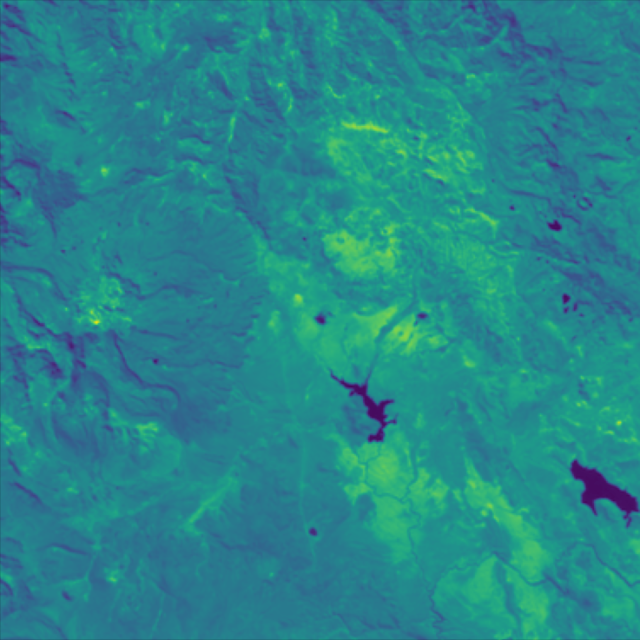
\includegraphics[width=\textwidth]{sample_nir_hr}
        \caption{High--resolution image}
    \end{subfigure}
    \hfill
    \begin{subfigure}{0.45\textwidth}
        \centering
        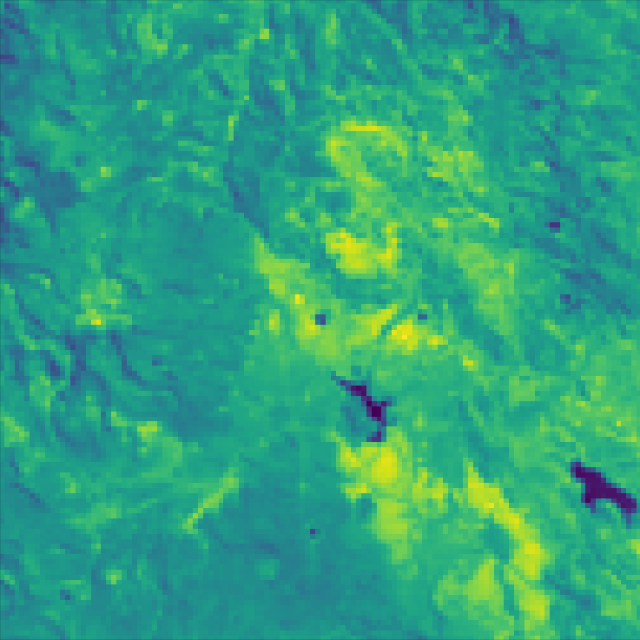
\includegraphics[width=\textwidth]{sample_nir_lr}
        \caption{Low--resolution image}
    \end{subfigure}
    \caption{Sample image pair from \textit{Proba--V NIR train dataset}}
    \label{fig:proba-sample}
\end{figure}
Furthermore, Proba--V features a set of binary masks for low--resolution images.
These masks indicate areas of photos that may not be suitable for processing, such as clouds or blank spaces.
An example of Proba--V image with a binary mask designating clouds is shown in the figure \ref{fig:proba_sample_mask}.
\begin{figure}
    \begin{subfigure}{0.45\textwidth}
        \centering
        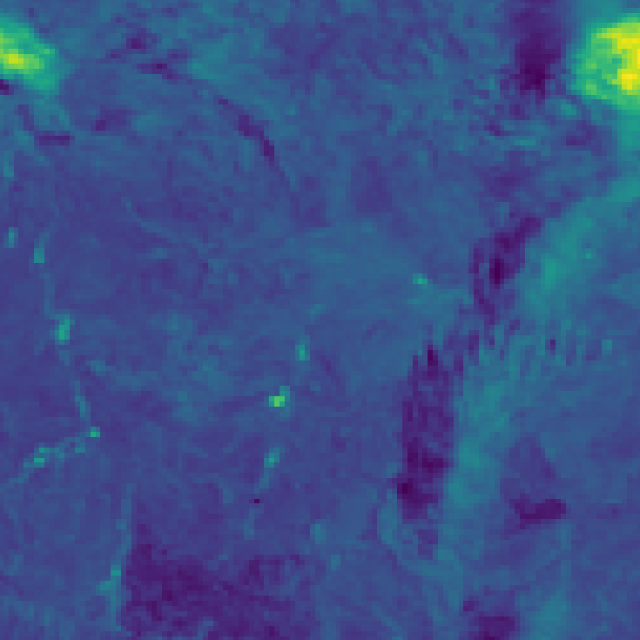
\includegraphics[width=\textwidth]{proba_sample_clouds}
        \caption{Sample Proba--V image with invalid area that contains clouds}
    \end{subfigure}
    \hfill
    \begin{subfigure}{0.45\textwidth}
        \centering
        
\includegraphics[width=\textwidth]{proba_sample_mask}
        \caption{Binary mask for a sample Proba--V image with invalid area}
    \end{subfigure}
    \caption{Proba--V sample with invalid area and its binary mask}
    \label{fig:proba_sample_mask}
\end{figure}

\subsubsection{Sentinel--2 as a super--resolution training dataset}
The super--resolution training part of the data demands can be met by utilizing \textit{Sentinel--2} dataset \cite{esa-sentinel}.
Contrary to Proba, it doesn't feature high and low--resolution scenes, for this reason, it suits the role of the dataset to undergo data generation process.
Sentinel--2 is part of a European earth observation programme that has lasted since 2015.
It gathers data from two twin satellites that acquire optical imagery at high spatial resolution from 10 to 60 meters.
Sentinel images are hyperspectral and feature a total of 13 bands.
Since it was decided not to include multispectral super--resolution only band eight is to be used (which is close to infrared).
A sample image from Sentinel--2 dataset is shown in the figure \ref{fig:sentinel_sample}.
\begin{figure}
	\centering
    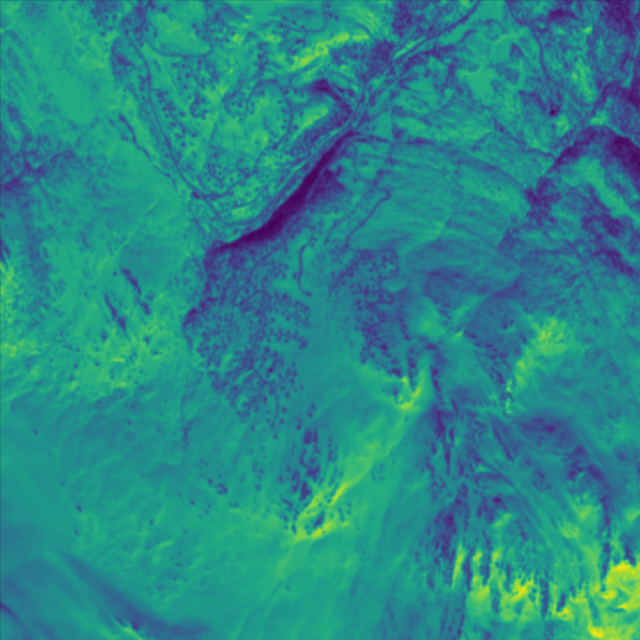
\includegraphics{sentinel_sample}
    \caption{Sample image from \textit{Sentinel--2 dataset} (eight band)}
    \label{fig:sentinel_sample}
\end{figure}

\subsubsection{Dataset for super--resolution evaluation}
Additional datasets are needed to evaluate final results.
The goal of the tests is to measure super--resolution generalization capabilities and data selection impact on the metrics.
This can be done in four ways with different data:
\begin{itemize}
	\item Each augmented Sentinel dataset should contain a test subset.
	\item Test subset generated in different ways can be tested in cross--validation scheme.
	\item Separate real--world Sentinel images can be used for tests. Sentinel doesn't include high and low--resolution pairs, so numeric tests are not possible. However, it is still viable to perform a visual test in search of artifacts.
	\item The Proba-V test subset used to evaluate the augmentation process can be used to measure super--resolution performance. Since the initial tests are not a part of any decision process, there is no information leak and the Proba subset can be used twice.
\end{itemize}

\subsection{Experiment flow}
Given the selection of data augmentation methods and available, data an experiment flow can be laid out in the form of a graph in the figure \ref{fig:experiment-flow}.
The graph follows the assumption of training various augmentation models with Proba--V dataset, exporting Sentinel--2 images for super--resolution training and final evaluation using cross validation and tests on real--world data.
\begin{figure}
	\centering
	\documentclass[tikz]{standalone}
\usepackage[utf8]{inputenc}

\usetikzlibrary{positioning}
\usetikzlibrary{shapes}
\usetikzlibrary{calc}

\begin{document}

\tikzstyle{cell} = [rectangle, rounded corners, minimum width=3cm, minimum height=1cm,text centered, draw=black, fill=white, align=center]
\tikzset{arrow/.style={-stealth}}

\begin{tikzpicture}[ampersand replacement=\&]
	\node[cell, fill=blue!20, align=center] at (1,0) (PVTS) {Proba-V train set \\(High and low-resolution pairs)};
	\node[cell] at (-5,0) (ANA) {Augmentation\\network achitecture};
	
	\node[cell, fill=blue!20] at (0.5,-2) (S2TS) {Sentinel-2 set\\(single-resolution)};
	\node[cell] at (-5,-2) (TAN) {Trained augmentation\\network};
	
	\node[cell] at (6,-2) (BIC) {Downsizing\\with bicubic interpolation};
	
	\node[cell, fill=blue!20] at (-1.5,-4.5) (SDTR) {Sentinel-2 degraded\\train set};
	\node[cell, align=center, fill=blue!20] at (-4.5,-5) (SDTS) {Sentinel-2 degraded\\test set};

\node[cell, fill=blue!20] at (6.5,-4.5) (SBTR) {Sentinel-2 bicubic\\train set};
	\node[cell, fill=blue!20] at (3.5,-5) (SBTS) {Sentinel-2 bicubic\\test set};
	
	\node[cell] at (1,-8.5) (HRNA) {HighRes-net\\architecture};
	
	\node[cell] at (6,-8.5) (HRNTB) {HighRes-net\\trained on bicubic};
	\node[cell] at (-4,-8.5) (HRNTD) {HighRes-net\\trained on degraded};
	
	\node[cell, fill=blue!20] at (-4,-11) (SR) {Sentinel-2 real test set\\(single-resolution)};
	\node[cell, fill=blue!20] at (6,-11) (PT) {Proba-V test\\(High and low-resolution pairs)};

    \path[arrow]
    (PVTS) edge (ANA)
    (ANA) edge (TAN)
    (S2TS) edge (TAN)
    (S2TS) edge (BIC)
    (BIC) edge (SBTR)
    (BIC) edge (SBTS)
    (TAN) edge (SDTR)
    (TAN) edge (SDTS)
    (SDTR) edge[bend right] (HRNA.north west)
    (SBTR) edge[bend left] (HRNA.north east)
    (HRNTB) edge[dashed] (SDTS) 
    (HRNTD) edge[dashed] (SDTS)
    (HRNTB) edge[dashed] (SBTS)
    (HRNTD) edge[dashed] (SBTS)
    (HRNA) edge (HRNTB)
    (HRNA) edge (HRNTD)
    (HRNTD) edge[dashed] (SR)
    (HRNTD) edge[dashed] (PT)
    (HRNTB) edge[dashed] (SR)
    (HRNTB) edge[dashed] (PT)
    ;
\end{tikzpicture}

\end{document}
	\caption{Graph of the experiment flow, solid lines indicate trainings, dashed arrows designate evaluations}
	\label{fig:experiment-flow}
\end{figure}

\section{Selection of tools and technologies}
\subsection{Language and libraries}
\textit{Python}, which is an industry standard for neural network research and scientific computing has been chosen as a main language for the implementation.
It combines ease of prototyping new code with efficient use of existing libraries written in more performant languages.
Python version 3.8 was chosen for the project as a reasonably recent, yet mature and field--tested version.

The main part of the work, consisting in writing neural network architectures and training them was written using \textit{Tensorflow} library.
Tensorflow has been a leading deep learning library in recent years and is widely used in the industry and academia.
The version 2.5 of the library was chosen for the project.
From the second version Tensorflow includes \textit{Keras} neural network prototyping interface natively as a default and recommended way for model building.
This work utilizes the Keras API as well as some underlying Tensorflow function for fine tuning and expanding models.
Tensorflow supports GPU acceleration via \textit{Nvidia CUDA} libraries, which is crucial for conducting efficient trainings.

The image manipulation tasks are performed using \textit{SciKit--image} library which offers a variety of IO functions, transformations and analysis tools.
\textit{Matplotlib}, another wide--spread Python library was used to create plots and heatmaps in the work.
Alongside SciKit--image, \textit{Pillow} was used for some image related operations (mainly for resizing images with specific interpolation modes).

\textit{NumPy}, the most popular numerical calculations library was chosen as a tool for matrix manipulation and mathematical operations.
Arrays created with NumPy are stored in contiguous memory layout, which enables utilization of performance optimizations such as vectorized operations. 
NumPy ubiquity in the world of scientific computing with Python proves to be very convenient.
It is compatible with other popular libraries; it is interoperable with parts of Keras API, Scikit--image stores images as NumPy arrays, Matplotlib can plot data from NumPy arrays out of the box.
NumPy arrays' performance comes from their static nature, their size is predetermined.
This constrain is prerequisite to the contiguous memory layout of the arrays, which enables utilization of fast mathematical operations.
However, this comes at a cost of flexibility; resizing the NumPy arrays is costly and often requires substantial memory reallocations.

The set of required libraries with proper versions can be installed using \textit{requirements.txt} files.
It is best to use it inside a Python \textit{virtualenv}, running the command: \mintinline[breaklines]{shell}{pip install -r requirements.txt}.

To ensure code quality and avoid mistakes, a \textit{continuous integration} system was used.
Continuous integration is based on automatic code building on the server with the help of version control systems.
Every time a new commit is pushed to the upstream, a set of checks is run remotely.
The integration system reports any errors which prevents integrating invalid code into the main system.
The built--in GitHub continuous integration and delivery system, called \textit{GitHub Actions} was used in the project.
Integration checks are performed inside a Ubuntu Docker image and consist of various \textit{flake8} linter analytics.

\subsection{Data and experiment management}
The codebase in the work was managed with \textit{Git} version control system.
Git is the most popular tool for tracking changes in code and text files.
However, it was not created with media and datasets in mind.
Git may work very slowly with large datasets and popular Git server providers such as \textit{GitHub} offer limited storage for repositories.
For this reason, \textit{dvc}---a supplementary tool was used.
\textit{Dvc} consists of two main components: data versioning and experiment tracking.
The data versioning part works similarly to systems like \textit{Git LFS}; it stores metadata inside the Git repository and the actual data in other storage (e.g. Google Drive).
Information about the proper data is stored in the form of \textit{MD5} hashes in the metadata files.
The metadata versioned with Git can be used to download proper data from the external cloud storage.
\textit{Dvc} is analogous to Git in operation, it uses a command line interface with a similar structure.
To download the data in the project one should run command \mintinline{shell}{dvc pull}.
Sine the metadata is versioned with Git, when going back in the commit history one should run \mintinline{shell}{dvc checkout} after \mintinline{shell}{git checkout} to conceal data versions.

The experiment tracking part of Dvc ensures reproducibility and result caching.
The layout of experiments is stored in the \textit{dvc.yaml} file where each stage of experiment is described with its input dependencies and outputs.
The results of each stage can be cached and rebuilt automatically depending on changes in the dependencies.
The experiments in this work usually depend on data and files with model architecture.
Training models can be parametrized using a configuration file, here named \textit{params.yaml}.
Parameters of models and training can be changed by editing this file.
Another convenience of dvc is that the outputs are automatically rebuilt on changes in the parameters.
Trained models are cached and bound with code and parameters used for training.
Similarly to the data versioning system, models and artifacts are also tracked with metadata and git.
When going back with history, \mintinline{shell}{dvc checkout} will also conceal artifacts and data.
The stage of the experiment pipeline is stored in the \textit{dvc.lock} file that also contains metadata.
The command \mintinline{shell}{dvc repro} is used to reproduce experiments.

Scripts in the project can also be run independent of dvc.
Training can be run with command: \mintinline[breaklines]{shell}{python -m cnn_res_degrader.train [-s] [-a] [-g] training_name} where the optional arguments decide which architecture to train and the positional argument is the experiment name.
The trainings done automatically by the Dvc system contain word \textit{dvc} as the experiment name.
Validation on Proba--V dataset can be run with command: \mintinline[breaklines]{shell}{python -m cnn_res_degrader.test [-s|-a|-g] weights_path output_dir} where the positional stores model architecture and positional arguments hold paths to trained model weights and output directory.

The augmented sentinel datasets can be created by running command: \mintinline[breaklines]{shell}{python -m export_sentinel.py [-s|-a|-g] [-r] [-d] weights_path}, where architecture and path to weights are denoted as described earlier.
The last two of the switches enable generating random translations, instead of using ones saved in sentinel files and running a demo export on one image instead of using the whole dataset.

\section{Project strucutre}
Files in the project have the following structure and function:
\begin{description}
	\item[.github/workflows/build.yml] continuous integration system configuration.
	\item[cnn\_res\_degrader] main part of the source code, contains the augmentation models, training and testing scripts.
	\item[dataset\_augmentation] source code for exporting augmented Sentinel--2 datasets.
	\item[data] super--resolution datasets and artifacts controlled by Dvc.
	\item[dvc.lock] metadata to track experiment progress in current commit.
	\item[dvc.yaml] dvc experiment description.
	\item[params.yaml] models and experiment configuration.
	\item[requirements.txt] libraries requirements.
\end{description}
Some configuration files and minor parts of project were omitted in this description.

\section{Additional remarks}
The following chapters will include many visualizations and image previews.
They often include a side--by--side comparison between high and low resolution images of the same scene that were generated using different methods.
When computers display single--chanel images (like the pictures presented in this work), a colormap is often used.
The most popular colormap is grayscale which displays white for max values, blacks for min values and shades of gray in between.
To improve visibility of details, a yellow and blue colormap called \textit{Viridis} is often used in this work.
Viridis is an example of a \textit{Perceptually Uniform Color Map}, which aims to guarantee an even perceived contrast of all color shades in the map.
However, when comparing a number of side--by--side images it is important to apply the colormap consistently across all pictures.
Modern image processing libraries may try to stretch colormap to the range of input image.
If images that are to be compared differ in maximal and minimal values, the way colormap is applied will be different.
It is important to ensure that images in the same scene display pixels with the same value in the same color.
For this reason, when several images are to be compared, they should be displayed with common colormap.
At the same time, an outlier pixel in one of the images can result in the colormap not being well suited to display the rest of the pictures.
The solution to choosing a good colormap range is to use maximum and minimum values using pixel mean values and standard deviation, as presented in the formula \ref{eq:colormap-maxmin}.
This way, only pixels within the range of three standard deviations from mean are taken into consideration when creating a common colormap for image comparison.
\begin{equation}
	c_{max,min} = \bar{p} \pm 3 \cdot \sigma_p
\label{eq:colormap-maxmin}
\end{equation}
  